\chapter{Analysis}
	
		
	\section{Verification of problem}\label{sec:verification}
		
 	\subsection{Green Space Benefits}
	It has been established that green spaces, like residential gardens or public parks and forests, provide ecosystem service benefits and have an impact on our psychological well-being and also physical well-being as they promote physical activity\cite{urbanGreenSpace}\cite{healthBenefitsNature}. Even though the urban public in cities, might not have private access to gardens if living in apartment buildings, and might therefore be forced to make use of the public green spaces, they still benefit from the ecosystem services from surrounding private yards\cite{greenSpaceBenefits}. As stated in the article \textit{How green is your garden?: Urban form and socio-demographic factors influence yard vegetation, visitation, and ecosystem service benefits}:\\
	
	\begin{quote}
		\textit{"Vegetation around the home can provide a variety of important ecosystem services that contribute to human and environmental health at local, neighbourhood, and regional scales\label{articleQuote}."}\\
	\end{quote}
	
	\todo{More on garden aesthetics leading over to landscape architects.}
	
 	\subsection{Who says so?}\label{whoSaysSo}
 	The design process of landscape architects has been heavily influenced by modern digital technology over the past 50 years, since Harvard's Laboratory of Computer Graphics was established.\cite{landscapeArchitectureDigiTech} In spite of landscape architects being first-movers in exploring digital applications for spatial analysis, many landscape architects are struggling with conceptualizing digital technology as a creative medium\cite{landscapeArchitectureDigiTech}. \\
 	\\
 	A survey on members of ASLA (American Society of Landscape Architects)\cite{surveySketchVSDigital}, shows that a 46\% of landscape architects prefer sketching by hand during the design process instead of using digital tools, 31\% prefer using a computer and the remaining 23\% use the computer for efficiency and the hand for creativity. Based on the statements given by the respondents the survey concludes that; \textit{"computers are not intuitive and design is intuitive"}\cite{landscapeArchitectureDigiTech}\cite{surveySketchVSDigital}. Although, computer software enables visualization in 3D which is an effective way of communicating large amounts of complex data to a wide non-expert audience, through visual cues that are more intuitive than those of a 2D-sketch, it can be time-consuming to create 3D visualizations\cite{landscapeVisual}
 	
 	\subsection{Why does it matter?}
 	
\begin{comment}
 	\subsection{Elderly people's approach to technology}
	 	Old people typically will not seek out to use state of the art technology, despite its ability to enable experiences that their age would otherwise prevent. As the elderly retire, they have more time on their hands to do whatever they feel like, and for some of these people gardening could be a very possible interest. But often, age lead to a loss of mobility, limiting old people's ability to garden and their enjoyment thereof, leading to a decrease in life quality. Professional teams have created immersive virtual reality applications like AlohaVR \cite{elderlyVRScout} to help people within the elderly age group seize their issues with chronic pain, relaxation, anxiety, and to provide general entertainment.
	 	%How does the below sentence relate to the above at all? Surely their lack of mobility has nothing to do with their ability to *design* a garden.
	 	So the question could be raised, would it be necessary to have a product that would function for garden designers to work with the elderly and including them in the technological experience? \\
 	
		
		The Pew Research Center has studied the technology adoption of elderly citizens in USA during the last 4 years. They created statistics \cite{seniorTechnology} to show the approach elders to technology as seen in \autoref {fig:oldstats1}. Furthermore the study shows estimates on actual use of different technologies by seniors in the age group 65+ years.
			\begin{figure}[H]
			\centering
			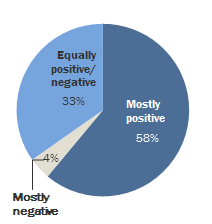
\includegraphics[width=0.4\linewidth]{figure/Analysis/oldpeoplestats1}
			\caption{Elderly peoples approach to technology in society.}
			\label{fig:oldstats1}
			\end{figure} 
		Another statistic shows how large a part of the senior population actually uses Internet and broadband as seen in \autoref{fig:oldstats2}. Nevertheless the graph shows that about 2/3 of the elderly population uses Internet to some extent, which allows the possibility for garden designers to design for the elderly. Furthermore these results creates the chance for garden designers to work with people of all ages, where earlier technology usually would be developed for the use with younger audiences and customers as they were the more common users.
			\begin{figure}[H]
			\centering
			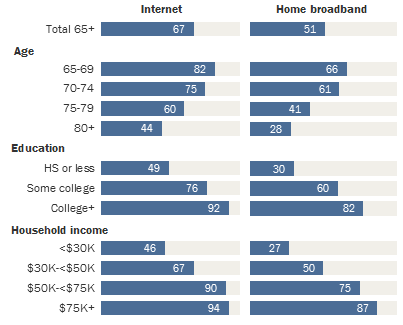
\includegraphics[width=0.6\linewidth]{figure/Analysis/oldpeoplestats2}
			\caption{Elderly peoples use of Internet and Broadband in percent.}
			\label{fig:oldstats2}
		\end{figure} 
	\end{comment}
		
	\subsection{Target Group}\label{sec:targetGroup}
	Evaluating the results of the ASLA survey as seen in \autoref{whoSaysSo} there seems to be an actual problem with creating 3D visualisations. It is far from impossible, but the time and effort it takes is non-beneficial for the landscape architects as these two factors, result in high cost in relation to time used on designing the visual landscape. \\
	The target group has been defined as \textit{Landscape architects}, and we needed to learn more about this target group. To this end, semi-structured interviews were conducted with different landscape architects. This way we would get a better understanding of both the target group and the context the product would be used in with the customers. The interviews were conducted via telephone and recorded for transcription, translation and analysis. The interview as a qualitative data gathering method, is to be analysed using the coding method to categorize statements from the targets.
	
	\subsection{Expert Interviews}\label{sec:expertInterviews}
	For further validation of the problem 4 phone interviews with landscape architects(Experts) were conducted. 2 of the experts were actively using 3D technology for visualizing garden plans for their customers. The other 2 only used sketching by hand to visualize their design for the clients. Due to logistics the interviews were conducted over the phone as the experts had their practises at various locations throughout Denmark. The interviews were semi-structured to allow for new ideas and points to potentially surface. Some practical advantages of interviewing over the phone instead of face-to-face interviews were also considered. These were, amongst others, advantages like Time Efficiency, (Re)arrangement Flexibility and Geographical Reach\cite{telephoneInterview}. 
		
		\subsubsection{Procedure:}
		This subsection is a brief description of how the interview process was executed.
		
		\paragraph*{Locating experts:}
		Through online research one project group representative found and e-mailed 12 landscape architects throughout the country and managed to make appointments with 4 of them. During the e-mail correspondence, the experts were informed, and gave their consent on the interviews being recorded and used in the report dependencies in transcribed form.
		
		\paragraph*{Preparation:}
		Through further online research a list of approximately 15-30 questions was compiled. The number depended on whether or not the expert used 3D in his/her practice, as this opened up for further questioning. Here are some examples of the questions:(See appendix \ref{sec:interviewQuestionsExperts} for the full list)

		\begin{itemize}
			\item[-] Do people usually need plans for the entire garden or just parts of it?
			\item[-] Who makes the 3D visualization of the garden? Is it something you create internally in the company, or does it come from outside cooperators? 
			\item[-] How large of a garden area do you usually work with?
			\item[-] Are your clients mostly private or do you also have municipal projects?
		\end{itemize}
		
		\paragraph*{Location:}
		As previously mentioned the interview were conducted over the phone. The interviewer was placed in a quiet room on campus at Aalborg University Copenhagen and made the phone calls to the experts at the agreed time.

		\paragraph*{Post analysis:}The expert interviews were later transcribed (See appendix \ref{interviewTranscriptions}) and coded using traditional coding in order to identify patterns and categorize followed by further analysis of the qualitative data gathered.
		
		\subsubsection{Findings}
		In this sub section the main categories from the previously mentioned coding process will be examined. In each category there will be translated quotes from the different interview, in no particular order. The list of categories is listed below:
		\begin{enumerate}
			\item Process
			\item Clients
			\item Design
			\item Technologies
			\item Resources
			\item Ideas
		\end{enumerate}
	
		\paragraph*{Process:}
		All of the experts were told to describe their process through a typical workday and how  much influence their customers had in the design process.
		\begin{quote}
			\textit{So when I show up at the customers house. I'm there for about 2 and a half hours and then we go in and out and I sit, and they tell me what their wishes are and I give some ideas}\label{quote:expertProcess1}.\\
		\end{quote}
	
		\begin{quote}
			\textit{It's not our opinion that should matter. We just tell them what they can and can't do and then they have to help us pick}\label{quote:expertProcess2}.\\
		\end{quote}
		
		\begin{quote}
			\textit{Yes, I really try to include them as much as I can. I have become more aware of how much I can affect them. [...] But now I listen more and more to what they really need. }\label{quote:expertProcess3}\\
		\end{quote}
		
		
		\paragraph*{Clients:}
		The experts were all asked about their clients and what kind of people they would usually work with. One thing they all had in common was that they would primarily work with private clients as oppose to municipal clients. And when asked about the ages of their clients, the answers varied. 
		
		\begin{quote}
			\textit{If it is private clients, then they are often from the mid-40's. 40’s 50’s, and there are also some older}\label{quote:expertClients1}.\\
		\end{quote}
		
		\begin{quote}
			\textit{In my experience it is people who bought a new house with 2 children. They are in their 30's. 30,32,35 and up, right? It is between 35 and 55-60}\label{quote:expertClients2}.\\
		\end{quote}
	
		\begin{quote}
			\textit{It's actually in the 20's. [...] Yes, there is a crazy amount in the mid-20's who are building houses}\label{quote:expertClients3}.\\
		\end{quote}
		
		\begin{quote}
			\textit{It's at least 40+, right? On Bornholm it can be younger}\label{quote:expertClients4}.\\
		\end{quote}
		

		\paragraph*{Design:}
		The experts were asked about different trends regarding garden design today, and compared to different places in Denmark or other countries, depending on their own experiences. We also asked in regards to special garden elements that the customers asked for.

		
		\begin{quote}
			\textit{There is actually far between that someone wants flowing water. You can say, sometimes someone wants a reflecting pool.}\label{quote:expertDesign1}\\
		\end{quote}
		
		\begin{quote}
			\textit{Yes, well you have to choose plants that can survive in the danish climate. Theres no hocus pocus in it. So... otherwise i dont think so. I don't know. That was a weird question. Haha. Well you can say about the coatings. Well I think those very light coatings they tend to get very very green and dark, right? So thats worth having a small seance about, but thats a very special thing to do.}\label{quote:expertDesign2}\\
		\end{quote}
		
		\begin{quote}
			\textit{But the trend is that it needs to be maintenance-free. That is at least on of the top points. It needs to be easy to maintain. And it needs to look very good, and it doesn't have to cost a million.}\label{quote:expertDesign3}\\
		\end{quote}

		
		
		
		\paragraph*{Technologies}



		\paragraph*{Technologies:}
		The experts using 3D visualization were asked about what software they used.
		\begin{quote}
			\textit{For us Google Sketchup is absolutely the easiest to work with. We have both also been running with AutoCAD before, and that is simply too heavy to dance with}\label{quote:expertTech1}.\\
		\end{quote}
		
		\begin{quote}
			\textit{Then I do a SketchUp drawing, that I continue working on in PhotoShop or some other way. And that is actually something that works fine for my type of assignments}\label{quote:expertTech2}.\\
		\end{quote}
		However, the experts not using 3D, were asked how come they did not use it.
		\begin{quote}
			\textit{Primarily it is because if I spend 2-3 hours on a garden, then I can't spend 2 hours on making something in 3D, because then it becomes a twice as expensive garden plan}\label{quote:expertTech3}.\\
		\end{quote}
		\begin{quote}
			\textit{I have this dialog so people can much better understand space because I explain about heights and everything. [...] And also because, if I were bring it home with me, then I would have to work with that every day. And that would be a too expensive process compared to what I sell to the customer}\label{quote:expertTech4}.\\
		\end{quote}
		


		\paragraph*{Resources}

		\paragraph*{Resources:}

		Even though some of the experts are spending time on creating 3D visualizations for their customers they could all agree that it is expensive.
		\begin{quote}
			\textit{If we have 80 on a year in total, then it is around 15 who get 3D. 15 out of 80}\label{quote:expertRessources1}.\\
		\end{quote}
		
		\begin{quote}
			\textit{In fact, I would assume that most people would do it, if it wasn't so much more expensive}\label{quote:expertRessources2}.\\
		\end{quote}

		\begin{quote}
			\textit{The reason that it is not use more is because it takes... It takes several days to create a good drawing. And 700 kr an hour times several days. Only the few are willing to pay that}\label{quote:expertRessources3}.\\
		\end{quote}
		
		\begin{quote}
			\textit{If it is over the top for me to say that a drawing like that should cost 7000, right? I think, well that is quite a lot of money, right?}\label{quote:expertRessources4}.\\
		\end{quote}
		
		\paragraph*{Ideas:}
		\begin{quote}
			\textit{Because, I already made the drawing. But could I have a 3D version made, that could be done so fast that I just made the finished sketch in 3D, then I think maybe it would be an upgrade, but then it doesn't have a plant list, then it is just the drawing in 3D. But that is the price range that I think could be interesting for me to work with}\label{quote:expertIdeas1}.\\
		\end{quote}
		
		\begin{quote}
			\textit{And it would be really good if you could make spatial representations easier, because then you would be able to use it much much more. Well, I would think that it would be fantastic, if I could send something to my regular customers, that I had not spent 3 days on making}\label{quote:expertIdeas2}.\\
		\end{quote}
	
		\begin{quote}
			\textit{Well ideally, then it would be that, when I in my process with the customer, in those 2 and a half hours, have been sitting and sketched to some result, then it would be super awesome. In some way it might just be that it was 3D that just stood up out of the paper}\label{quote:expertIdeas3}.\\
		\end{quote}
		
		\begin{quote}
			\textit{And if you could put on some glasses and the draw out in the air}\label{quote:expertIdeas4}.\\
		\end{quote}
		
		\subsubsection{Sub-conclusion}
		The landscape architects usually include their clients in the design process and therefore it would be relevant to consider these clients as a secondary target group. Based on the client related questions it is clear that the target groups primary customers range from around 25 to 60 years. There are no distinctive design elements that are heavily used. The trends are that the gardens should be maintenance-free and have plant that is able to survive the Danish climate due to shifting weather through the year.
		Even though some landscape architects use 3D visualization it has to be an easy and efficient process in order to keep the cost down. Otherwise the customers will probably do without it.
		

	\section{Context}
	The context is to provide useful CAD style virtual reality software for landscape architects. In order to know what is useful to them, it must be concluded what the needs and what problems actually occurs to landscapes architects, and in that regard how an immersive VR software could help them design with and/or without their customers. Also it needs to be beneficial for the landscape architect to use the software, to consume less time, effort and money, which the goal of making the process of designing a garden go with ease rather than frustration due to complex software or the like. \\
	
	Furthermore, it must be known which current technologies are used in the field, to comprise needed features and find what needs to be excluded in the developing process. Nevertheless, investigation on how immersive virtual reality works in general should be done. This includes which benefits it brings to modern engineering works and how virtual reality development is maturing in that regard.
			
	\section{Technologies}\label{sec:technologies}			

			\subsection{Fiducial markers}\label{sec:fiducialMarkers}
				By measuring fiducial marker systems, regarding their performance, it is possible to rate the markers by how reliably it finds vpoints matching physical points on the markers. There can be several reasons to why a fiducial marker system would have problems working or live up to the desired performance. This is typically; poor tolerance to lightning conditions and cluttered scenes causing similar markers to be mistaken by each other\cite{fiducialMarkers}. These problems may complicate the system design.\\
				
				There are however a way to figure out if the fiducial marker system is useful and reliable. This can be characterized by some numerical metrics and some qualitative observations, made with carefulness;\\
				\begin{enumerate}
					\item the false positive rate,
					\item the intermarker confusion rate,
					\item the false negative rate,
					\item the minimal marker size,
					\item the vertex jitter characteristics,
					\item the marker library size,
					\item immunity to lighting conditions,
					\item immunity to occlusion,
					\item perspective support,
					\item immunity to photometric calibration, and
					\item the speed performance.\\
				\end{enumerate}
				
				Failing to properly address these criteria will reduce the usability of a marker system remarkably\cite{fiducialMarkers}. All of the numbers have a valid reason for them to be announced; The false positive rate is falsely reporting the presence of a marker when none is present. The intermarker confusion rate is when one marker is mistaken for another. The false negative rate is when the marker can be seen on an image, but not reported. The minimal marker size is the size of the pixels required for the system to detect the marker. The vertex jitter is the noise in the marker corner positions. The library size is the number of unique markers the system is capable of storing. Two important things from the list is immunity to lightning conditions and immunity to occlusion, for a fiducial marker system it is crucial that the system is able to detect and recognize the markers despite the ambient lighting and partial covering of the pattern.\\
				Last is to mention the practical issue of speed performance. A vision-based fiducial marker tracking system must function in real time, using a low cost computing power, for it to be considered useful.\\
				
				All these criteria can be highly fulfilled using a system called ARTag \cite{fiducialARTag}. ARTag consists of a library of patterns with a square border and unique interior digital signature, along with the possibility to detect algorithms found in imagery \cite{fiducialMarkers}.\\
				
				It is important to state here, that not every kind of pattern in a marker is suitable when it comes to fiducial markers\cite{fiducialMarkers}. As an example it is worth mentioning bar codes as seen in \autoref{fig:fiducialmarkers}, these are not suitable as fiducial markers, because they are made to be read by a laser scanner.\\
				Alongside bar codes follows QR. There are two reasons for this; in fiducial marker systems a large field of view is usually preferred. therefore QR is not suitable for this, mainly because they are not intended for this kind of system.This will cause perspective distortion and they will not provide enough image points for 3D pose calculation.The second reason that QR is not suitable is because they require a large area in the image, this will limit the range as to where the markers can be used.\\ 
				
				
					\begin{figure}[H]
						\centering
						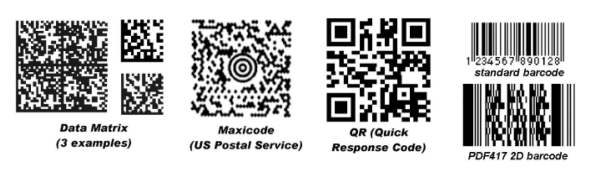
\includegraphics[width=0.9\linewidth]{figure/Analysis/fiducialmarkers.png}
						\caption{Different markers, not suitable for a fiducial marker system.}
						\label{fig:fiducialmarkers}
					\end{figure}
					
				
				As stated above, there are a lot of different markers that can be used for a fiducial marker system, but some are more efficient than others, depending on what kind of system will be used.
				Fiducial marker systems is usually functioning in two different stages; hypothesis generation and verification/identification.\\
				
				To test the pattern, six parameters are still necessary. The perspective projection has to be approximated by a parallel one. For this, a first stage must find candidate regions by locating one or more relatively unique features of the marker this is because the space of possible homographies or parallel transforms is too large to test an image for valid patterns by exhaustive search \cite{fiducialMarkers}.
				A geometric shape or shapes, such as a dot, bar, ellipse, triangle, square, etc., provides an anchor to form a marker detection hypothesis.\\
				
				Moving on to second stage, but with some important notes from stage one, such as; homography or parallel parameters, which checks if the region is actually a marker or just an object in the environment. As prior mentioned regarding coded dot systems, a parallel warp can be calculated on the ellipses major and minor axes.
				as seen in \autoref{fig:fiducialworking}, several marker systems is shown and they all presume planarity and use a parallel or homography mapping.
				
					\begin{figure}[H]
						\centering
						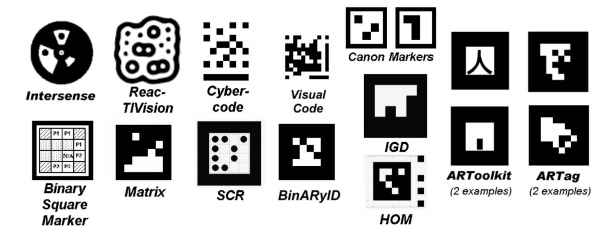
\includegraphics[width=0.9\linewidth]{figure/Analysis/fiducialworking.png}
						\caption{Different markers, suitable for a fiducial marker system.}
						\label{fig:fiducialworking}
					\end{figure}
					
				It is unlikely to find a marker system that does not use any kind of thresholding, connectivity or blob analyses/detection, this is due to details. Though using thresholding and connectivity does not come without some error modes. How well the first stage is implemented affects the false negative detection rate. this is due to incorrect thresholding, which leads to markers that will be missed. Minimal marker size, vertex jitter characteristics, and especially immunity to
				lighting conditions\cite{fidOcclusion} are also something that has to be considered.\\
				
				A system using only parallel mappings will have trouble with larger markers as well as cameras with a small focal length; for example Webcams(in laptops or portable ones) and cameras built into portable devices.
				 
				
				
				
			\subsection{Image Processing}
		
			Image processing is the act of enhancing, or extracting information from, a digital image using certain operations. It will take as input a photograph, computer generated image, or even a video feed, and return an output depending on the operations performed. Visual enhancements could be brightening a scene, increasing color saturation, or resizing, flipping, twisting and turning the image. Information extracted from the frame could be  in the form of counting objects or identifying objects, even complicated ones like faces. 
		
			\subsubsection{Color detection}
			
			One of the simpler things to extract from an image is color. A simple program may count the number of pixels with the RGB color code (255,0,0), which we know as "red". A slightly more sophisticated program will have some leniency built in, counting red-ish colors as being red. This is useful since in a real life scenario, neither the camera nor the light is going to be perfect, and therefore some inaccuracies must be accounted for. 
			
			The ideal color space to use for color detection depends on the specific case. 
			%insert pictures of color spaces
			For example, given the below image of leukocytes (white blood cells) surrounded by other blood cells, which color space would be most suitable for extracting the leukocytes?
			\begin{figure}[H]
				\centering
				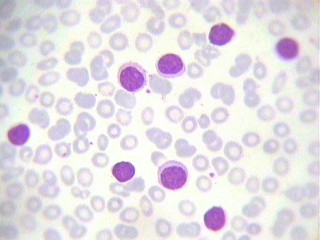
\includegraphics[width=0.2\linewidth]{figure/Analysis/leukocytes.jpg}
				\caption{White blood cells (Purple cells in image)}
				\label{fig:leukocytes}
			\end{figure}
			
			By converting the image to different color spaces and separating each space into its components, we can see in which channel of which color space the desired objects stand out the most. 
			
					\begin{figure}[H]
				\centering
				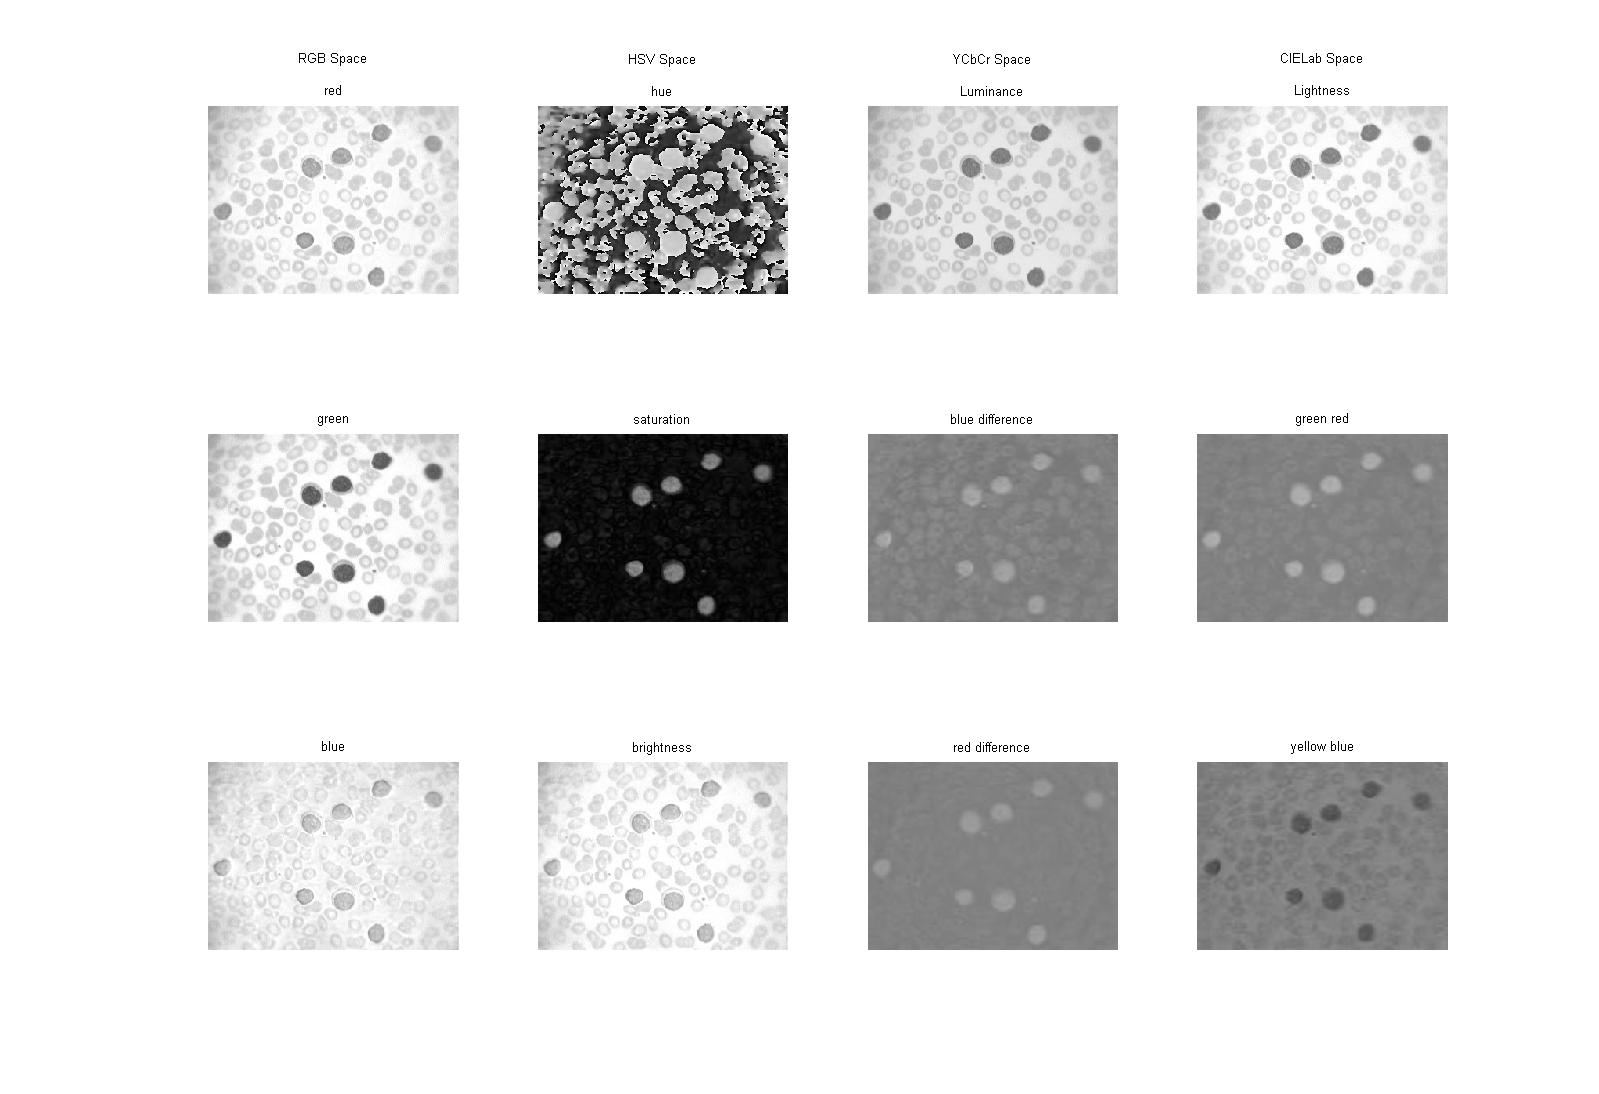
\includegraphics[width=\linewidth]{figure/Analysis/differences.jpg}
				\caption{Color space differences}
				\label{fig:differences}
			\end{figure}
		%Images from https://stackoverflow.com/questions/30022377/should-i-use-hsv-hsb-or-rgb-and-why
		Here we see that the leukocytes stand out the most in the saturation channel of the HSV color space. But they are also quite noticeable in the green channel of RGB space. It would likely be the best option to use HSV in this case. 
		
			\subsubsection{Edge detection}
			
			Edge detection is performed by applying a variety of mathematical methods. Simply put the algorithm will find points in a digital image in which the brightness changes abruptly. 
			
			\subsubsection{Blob detection}
			
			A BLOB, or "Binary Large OBject", refers to a group of connected pixels in a binary image. Detecting BLOBs in an image must be done before we can start analyzing and comparing their features. Examples of such features could be area, compactness, circularity, or center of mass.
			
			In order to make an image binary (each pixel being either completely black or completely white), a thresholding operation must be performed. The parameters of this function will greatly affect the resulting image to be processed. 
			
			Defining distinct BLOBs in a binary image is accomplished by going through the image one pixel at a time until a non-zero (foreground) pixel is found. One method is to now check the pixel's neighbors for connected foreground pixels, and so recursively check every neighbor's neighbor until the entire collection of pixels are assigned to the same object. This is called the grass-fire algorithm. Another method doesn't check recursively, instead requiring a second pass to correct certain BLOBs being classified as multiple objects.
			
			
			\subsubsection{Object recognition}
				Having extracted features from the detected objects, those features can be compared to those of pre-defined objects to determine if they match. A simple implementation might compare the color and circularity of an object to that of a perfectly round, red circle. 
				
				More advanced object recognition relies on deep learning algorithms, in which the program analyzes a digital catalog of object examples in order to define which parameters best define a particular type of object.
			

		\subsection{Assessment of Virtual Reality software in engineering}
		Human-Computer interfaces are traditionally known to be controlled using devices like the mouse and keyboard, while actions are monitored on computer monitors, which could be perceived as unnatural in a regard, as it does not act well with the human senses as they are used. However, with the development over time of modern technology, it has come across Virtual Reality (VR). \\
		
		Virtual reality uses what is known from the human-computer interface and implements it in a structure that activates and increases the users human senses. A typical virtual reality device uses a Head Mounted Display with a stereoscopic display and can eventually feature audio. Furthermore, it sets the user in a place that gives them the sense of actual presence in the environment they are put into. The display is split into right-eye and left-eye views to mock the feeling of stereoscopic human vision while wearing the display. 
		
		Another issue with virtual reality and the immersion of actual reality, how force feedback is processed enable the user to actually feel if they e.g. touch something, hear anything etc. This issue is resolved through the use of Haptic feedback e.g. bHaptics TactSuit\footnote{bHaptics TactSuit: \url{http://www.bhaptics.com/tactsuit.html}} \\
		
		In engineering VR software was developed using existing libraries most commonly from C or C++. The libraries were designed with functions to track data coming from the user input e.g. rotation. With these libraries engineers in history built toolkits to make virtual reality engineering accessible for development in regard to actual requirements of the single user. \cite{engineeringVR}
		In modern engineering engines like Unity using C\# scripts and custom plug-ins allows for fast visualization of models or environments in virtual reality. With the use of Unity and the virtual machine C\# uses, more users have access to experiencing virtual reality applications made in the engine. With the high accessibility engineering works in virtual reality, it has become more natural, in the aspect that an engineer could be present in a virtual space, whilst designing, shaping or in anyway creating physical objects but in virtual space. The major benefit of this is the cost, it is not very expensive, as the software provides materials, tools and all the things usually needed to be bought from hardware stores etc. before creating actual designs. \\ 
		
		Virtual reality allows for early and precise visualizations of conceptual designs, which could be for any sort of profession e.g. architecture, plumbing, carpentry and the like. Besides conceptual design, it has also been used for manufacturing planning where one could track the process of assembling objects, machines etc. to plan what effort goes into the process of manufacturing. It can be understood as a Computer Aided Design (CAD) software, but as mentioned in \cite{engineeringVR} with the immersive feel. This means that the user actually activates and uses several human senses in the process of any of the aforementioned situations. As engineers have been using regular CAD software for decades, most of them are familiar with the interface, and that should not be much of a concern when developing VR CAD software.

									
		\subsection{Virtual Reality}
		The earliest attempts at a VR experience was in the 1950s\cite{VRS} by Morton Heilig who made the Sensorama\ref{fig:sensorama}; an arcade-style theater cabinet, that featured stereo speakers, stereoscopic 3D display, smell generators, fans and a vibrating chair.
		\begin{figure}[H]
			\centering
			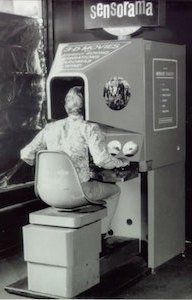
\includegraphics[width=0.4\linewidth]{figure/Analysis/sensorama2}
			\caption{The Sensorama made by Morton Heilig in the 1950s. Fully featured first step at virtual reality.}
			\label{fig:sensorama}
		\end{figure}
		There were a couple of short movies made for the Sensorama, but these were all produced and edited by Morton Heilig himself. The whole setup was stationary, and didn't feature any Head Mounted Display (HMD), so the user had to sit in the vibrating chair and look straight at the display for the duration of the movie. The more modern versions do not include features like smell and fans, but are also geared more towards mobility and full body immersion, and having a vibrating chair doesn't promote that idea.\\
		
		Morton Heilig later went on to further develop the idea of virtual reality, by making the first HMD in form of the Telesphere Mask\cite{VRS} in 1960. This took the immersive nature of his first product to a more personal level, even though it still just were a simple stereoscopic 3D wide view, with stereo sound. It did however look more like the virtual reality headsets of the modern day as seen in \autoref{fig:telesphere}.
		\begin{figure}[H]
			\centering
			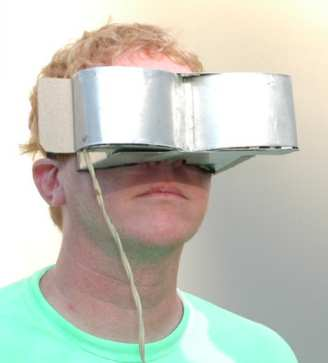
\includegraphics[width=0.25\linewidth]{figure/Analysis/TelesphereMask}
			\caption{The first attempt at HMD virtual reality headset, made by Morton Heilig in 1960. It worked by having stereoscopic 3D vision and stereo sound.}
			\label{fig:telesphere}
		\end{figure}
		Even though it was a step in the direction of a functioning virtual reality headset, it was still only a display showing a movie, it didn't have any motion tracking, or interaction between the user and the movie being watched. There was a sore lack of immersion, which is what makes the virtual reality headsets of today what they are.\\\\
		
		In 1961 the first motion tracking HMD was developed\cite{VRS}, it was made for military purposes, and was focused on tracking the head movements to control a remote camera. This was to allow a soldier to view remote locations in a natural fashion, without risking the viewer to actually be physically present. It used magnets to accomplish the head motion tracking.\\
		
	
	
		After the initial excitement for virtual reality died down with the invent of the world wide web in the mid 90's, the industry waited patiently for hardware that could provide the immersion that tied the experience as a whole together. All of the early attempts had one flaw in common; the hardware couldn't provide close to realistic or good looking graphics at a frame rate that wouldn't induce motion sickness in the user, at a price that a normal consumer could afford\cite{vergeVR}. And hence the virtual reality industry laid dormant until 2013 when Palmer Luckey created a kickstarter page for a virtual reality headset called Oculus Rift\cite{createOculus}. This headset sparked a wide public interest in virtual reality as a medium, and lead to the development of the current selection of VR headsets available today. The most current iteration of the Oculus Rift is the CV1 - Consumer Version 1. Its biggest competitor is the HTC Vive, a VR headset with similar hardware specifications\footnote{Vive™: \url{https://www.vive.com/us/}}.
	
		
		\subsubsection{Standalone VR}
		Oculus Go\footnote{Oculus Go: \url{https://www.oculus.com/go/}} is a virtual reality headset set to launch in the first quarter of 2018. Developed by the firm behind Oculus Rift, the Go shares many features with the Rift. It is designed for virtual reality games, social applications and different kinds of 360 degree experiences. Furthermore, the Go is constructed of lightweight fabrics which increase comfort during long sessions of use. Unlike the Rift, Oculus Go does not need to be connected to a computer in order to function, enabling it to be used in new contexts such as outdoors and while traveling. It utilizes a simple controller for navigation and action to allow complex interaction within the featured applications, although it does not feature fully tracked motion control. Another strength the Go brings is the built in spatial audio, which alongside the 2560x1440 pixel display makes the Oculus Go a serious competitor to current mobile VR headsets.  \\
		\begin{figure}[H]
			\centering
			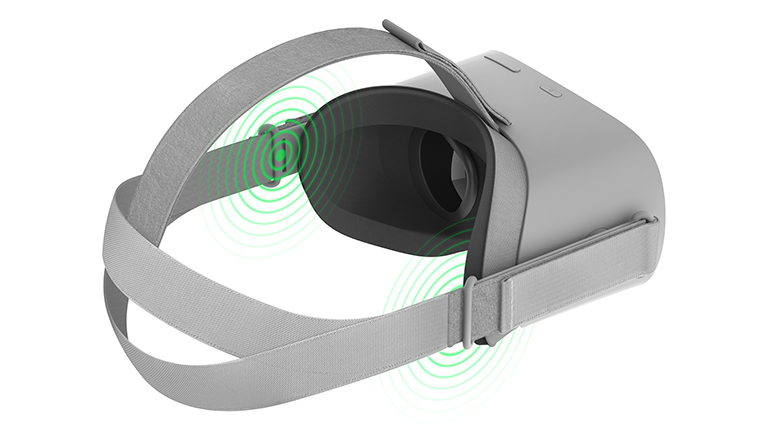
\includegraphics[width=1.0\linewidth]{figure/Analysis/oculusgo}
			\caption{The Oculus Go concept preview}
			\label{fig:Oculus}
		\end{figure}
		
		At the time this report is written, the product is not yet commercially available. Organizations developing for the headset may apply for an early version of the hardware to develop on. It is however possible to develop an application for the Go without owning one, as the Go is directly compatible with applications designed for GearVR. 
		
		Oculus Go is not the only standalone VR headset in the works. Google is working with Lenovo on Daydream, and HTC is developing the Vive Focus, a portable alternative to the HTC Vive. Little information is available about the release date of either product, and the latter is set for a China-exclusive launch. As such, GearVR and Oculus Go are the only current options for portable VR development. \todo{do we need sources here?}
		
		
		\subsubsection{The essence of VR}
		Virtual reality is a medium\cite{definingVirtualReality} that has been a long time underway. Starting in the sixties, and reemerging as a popular technology 2013, this medium is usually defined by a set of hardware implementations. These hardware implementations range a lot in price and devices, but a broad definition of the medium is:\\
		
		\begin{quote}
			\textit{Virtual Reality is electronic simulations of environments experienced via head-mounted eye goggles and wired clothing enabling the end user to interact in realistic three-dimensional situations}\cite{coates1992}.\\
		\end{quote}
		
		This definition is however quite old, being from 1992, but it does still apply to a certain degree to the current state of virtual reality as a device specific medium. Even though the devices, and their capabilities have changed, the way of interaction with the medium is largely the same; Put on a head mounted display, grab the controllers, and explore the 3D world you put yourself into. The rest of the paper will assume the definition of virtual reality as being:\\
		\begin{quote}
			\textit{Virtual Reality is electronic real time simulations of environments experienced via head-mounted eye goggles and one or more controllers enabling the end user to interact in realistic three-dimensional situations}\label{def:virtualRealityDefinition}.\\
		\end{quote}

    \section{State of the art}\label{sec:SOTA}
	  
		\subsection{VR Gardens}
			VR Gardens is a mobile application for designing and planning your own garden. It contains a variety of different 3D models of trees, bushes, outdoor furniture, tiles and the like, to help visualize any garden idea one might have. The design can then be reviewed using the Google Cardboard\footnote{Google Cardboard: \url{https://vr.google.com/cardboard/}} or similar simple Virtual Reality boxes to be immersed in a close-up edition of the design.
			\begin{figure}[H]
				\centering
				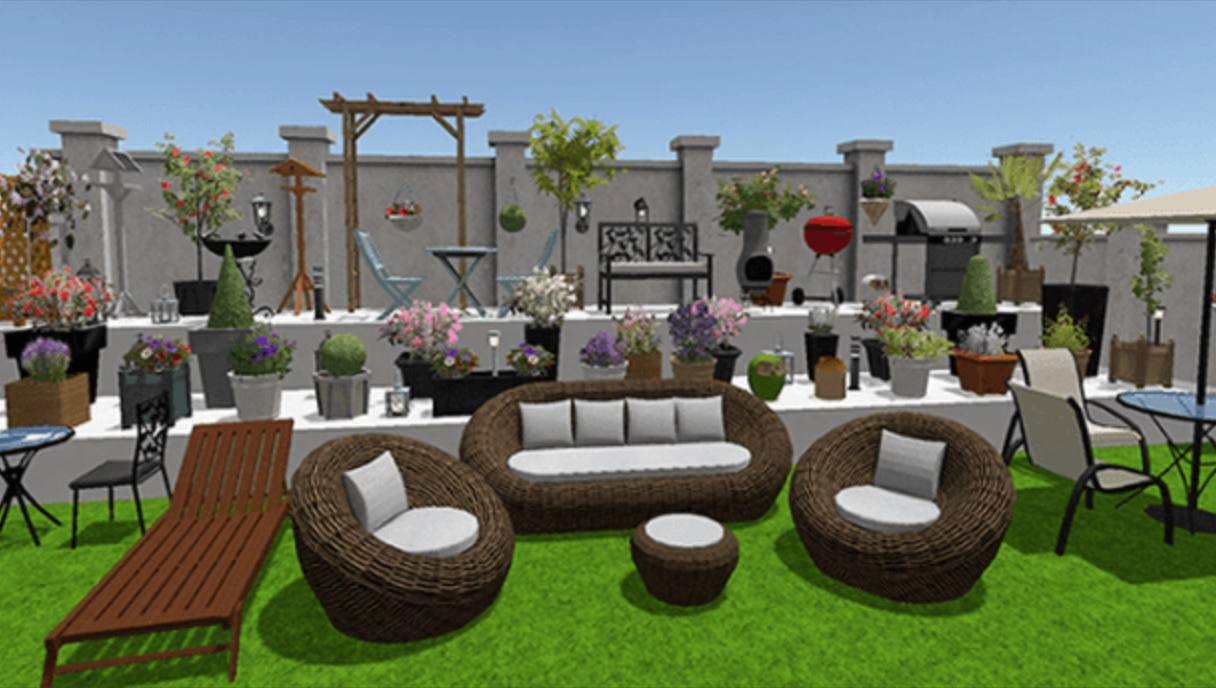
\includegraphics[width=0.6\linewidth]{figure/Analysis/vrgardens}
				\caption{VR Gardens comes with many pre-rendered 3D models}
				\label{fig:vrgardens}
			\end{figure}
			Although, because of the many functions of the application, it is also quite complex, and seems to have a rather steep learning curve. It is almost focused entirely on mobile as well, the web application implementation is just a ported version of the mobile application. Doing it exclusively on mobile is helping make it more agile, but is also limiting the capabilities of both interface and hardware. The limited screen space has made the interface very compact and the controls feels clunky with touch. The effort can be noticed throughout the use, but ultimately the experience falls short due to the 	platform choice.
			
		\subsection{Invita kitchen VR}
			The danish kitchen interior design business Invita, has made it possible for their costumers to experience their new kitchen in 3D with a set of VR goggles \footnote{Invita VR kitchen: \url{http://www.invita.dk/kampagne/virtual-reality/}}. This gives the customer the option to see their new kitchen "in real life" before they go ahead and buy it. To ensure that the customer picks out the perfect kitchen for them, they now have the opportunity to se multiple kitchens before making a final decision.\\
			To get an idea of how it works, and how the interior designers make this happen, the costumer must make an appointment with Invita's designers before it is possible to see the process and the outcome of the desired design.\\
			This procedure is a great example of the development of using 3D space combined with VR and what benefits it has for the future of companies, especially ones where VR is an obvious solution. Invita has made it easier to show off their kitchens, and the costumer get a much greater feeling regarding which kitchen they want to purchase afterwards. This prevents the costumer to regret their decision after they purchase the kitchen, which draws a perfect parallel to our Garden VR design. The costumer can choose between different elements in their garden, before settling on one specific thing. It will also make it easier for the designer, they have all the elements they need in their 3D program, therefore it is up to the costumer too decide which elements they want in their garden/kitchen.

			
		\subsection{Mental Canvas}
			A software system that combines 2D draw-and-paint with 3D\footnote{Mental Canvas: \url{https://www.mentalcanvas.com}} which enables a user to create a 3D environment from sketches, supporting conceptual architectural design and analysis. It has been created for Microsoft's Surface technologies\footnote{Microsoft Surface: \url{https://www.microsoft.com/en-us/surface}} and is compatible with the Surface Dial. The system allows for the user to place 2D surfaces, or \textit{canvases} in a 3D space using traditional CAD(Computer-Aided Design) tools of positioning, scaling, rotating on XYZ-coordinate axes.\cite{sotaMentalCanvas}
			
				\begin{figure}[H]
					\centering
					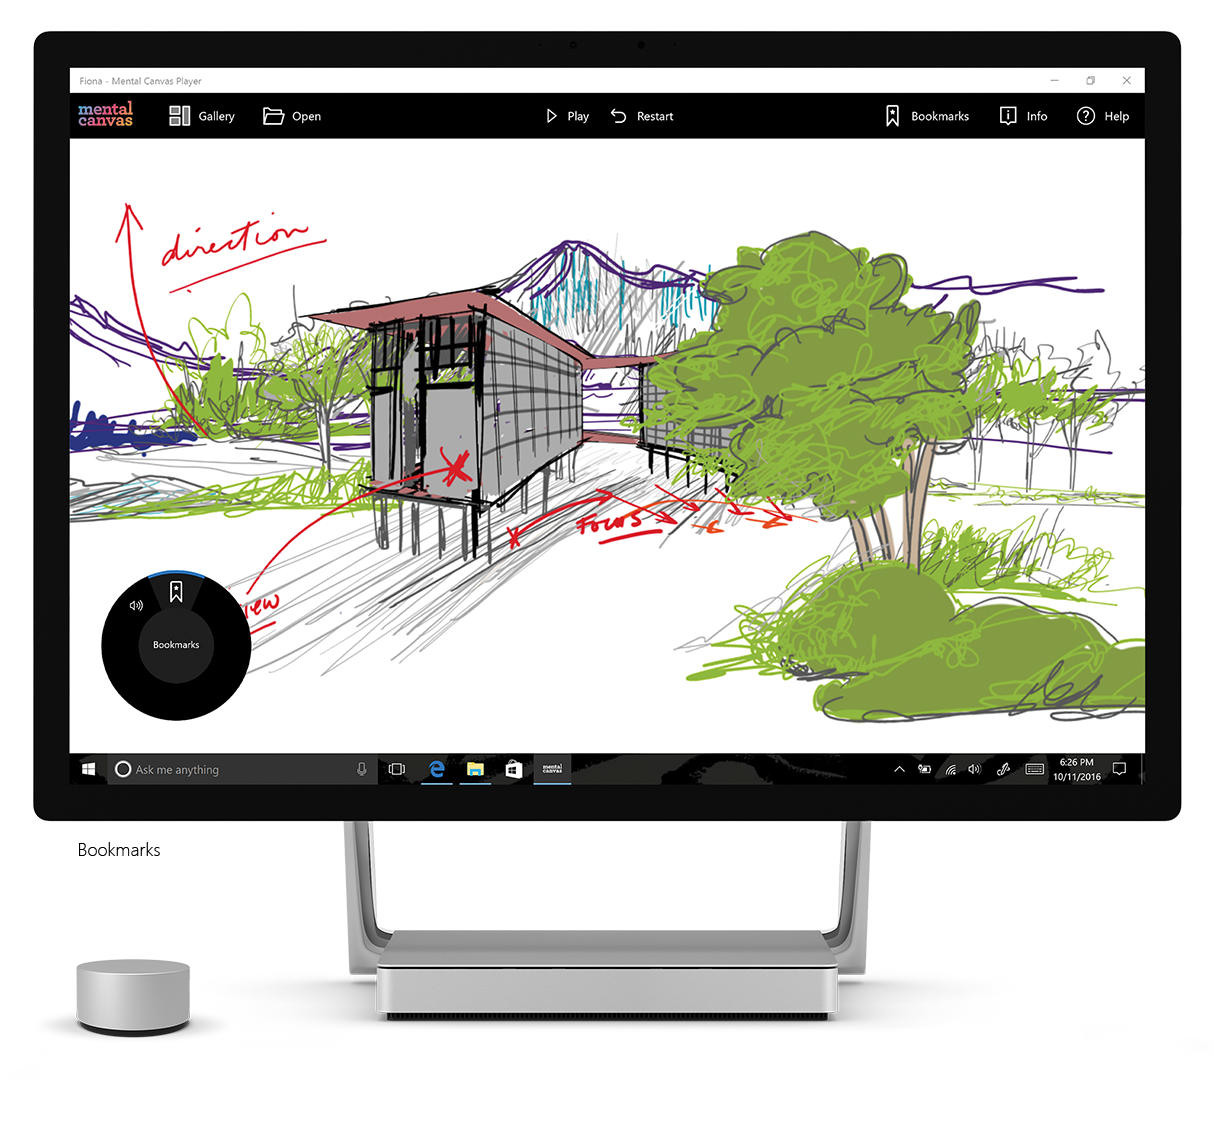
\includegraphics[width=0.5\linewidth]{figure/Analysis/mentalCanvas.png}
					\caption{Mental Canvas combines 2D sketching systems with 3D computer systems.}
					\label{fig:mentalCanvas}
				\end{figure}

		\subsection{Reactable}
			reacTIVision\footnote{reacTIVision: \url{http://reacTIVision.sourceforge.net/}} is a framework for developing computervision applications and interfaces. It uses fiducial markers as seen in  \autoref{sec:fiducialMarkers} to sense objects and movement, which allows for more extended interaction. It also makes use of the TUIO protocol, which is a protocol used for tangible multitouch surfaces, this means that it is enabled to take input from multiple tagged objects through a sensor, and send messages from the tracker to the client application. \\
			
			Reactable\footnote{Reactable: \url{http://reactable.com/}} is a musical instrument that uses the reacTIVision framework, to map different midi-controllers on a tabletop interface. The different types of fiducial markers displayed on cubes or small figures work as knobs, buttons and the like to imitate an analogue synthesizer, but with different types and more visual interactions. It enhances the musician's or sound engineer's chance to be more visually creative with their music. The table itself consists of a camera/sensor at the bottom pointing upwards to the tabletop. The sensor detects interactions made by the user and how the fiducial markers are altered over time, which results in the creation of a a musical sound space.
				
				\begin{figure}[H]
					\centering
					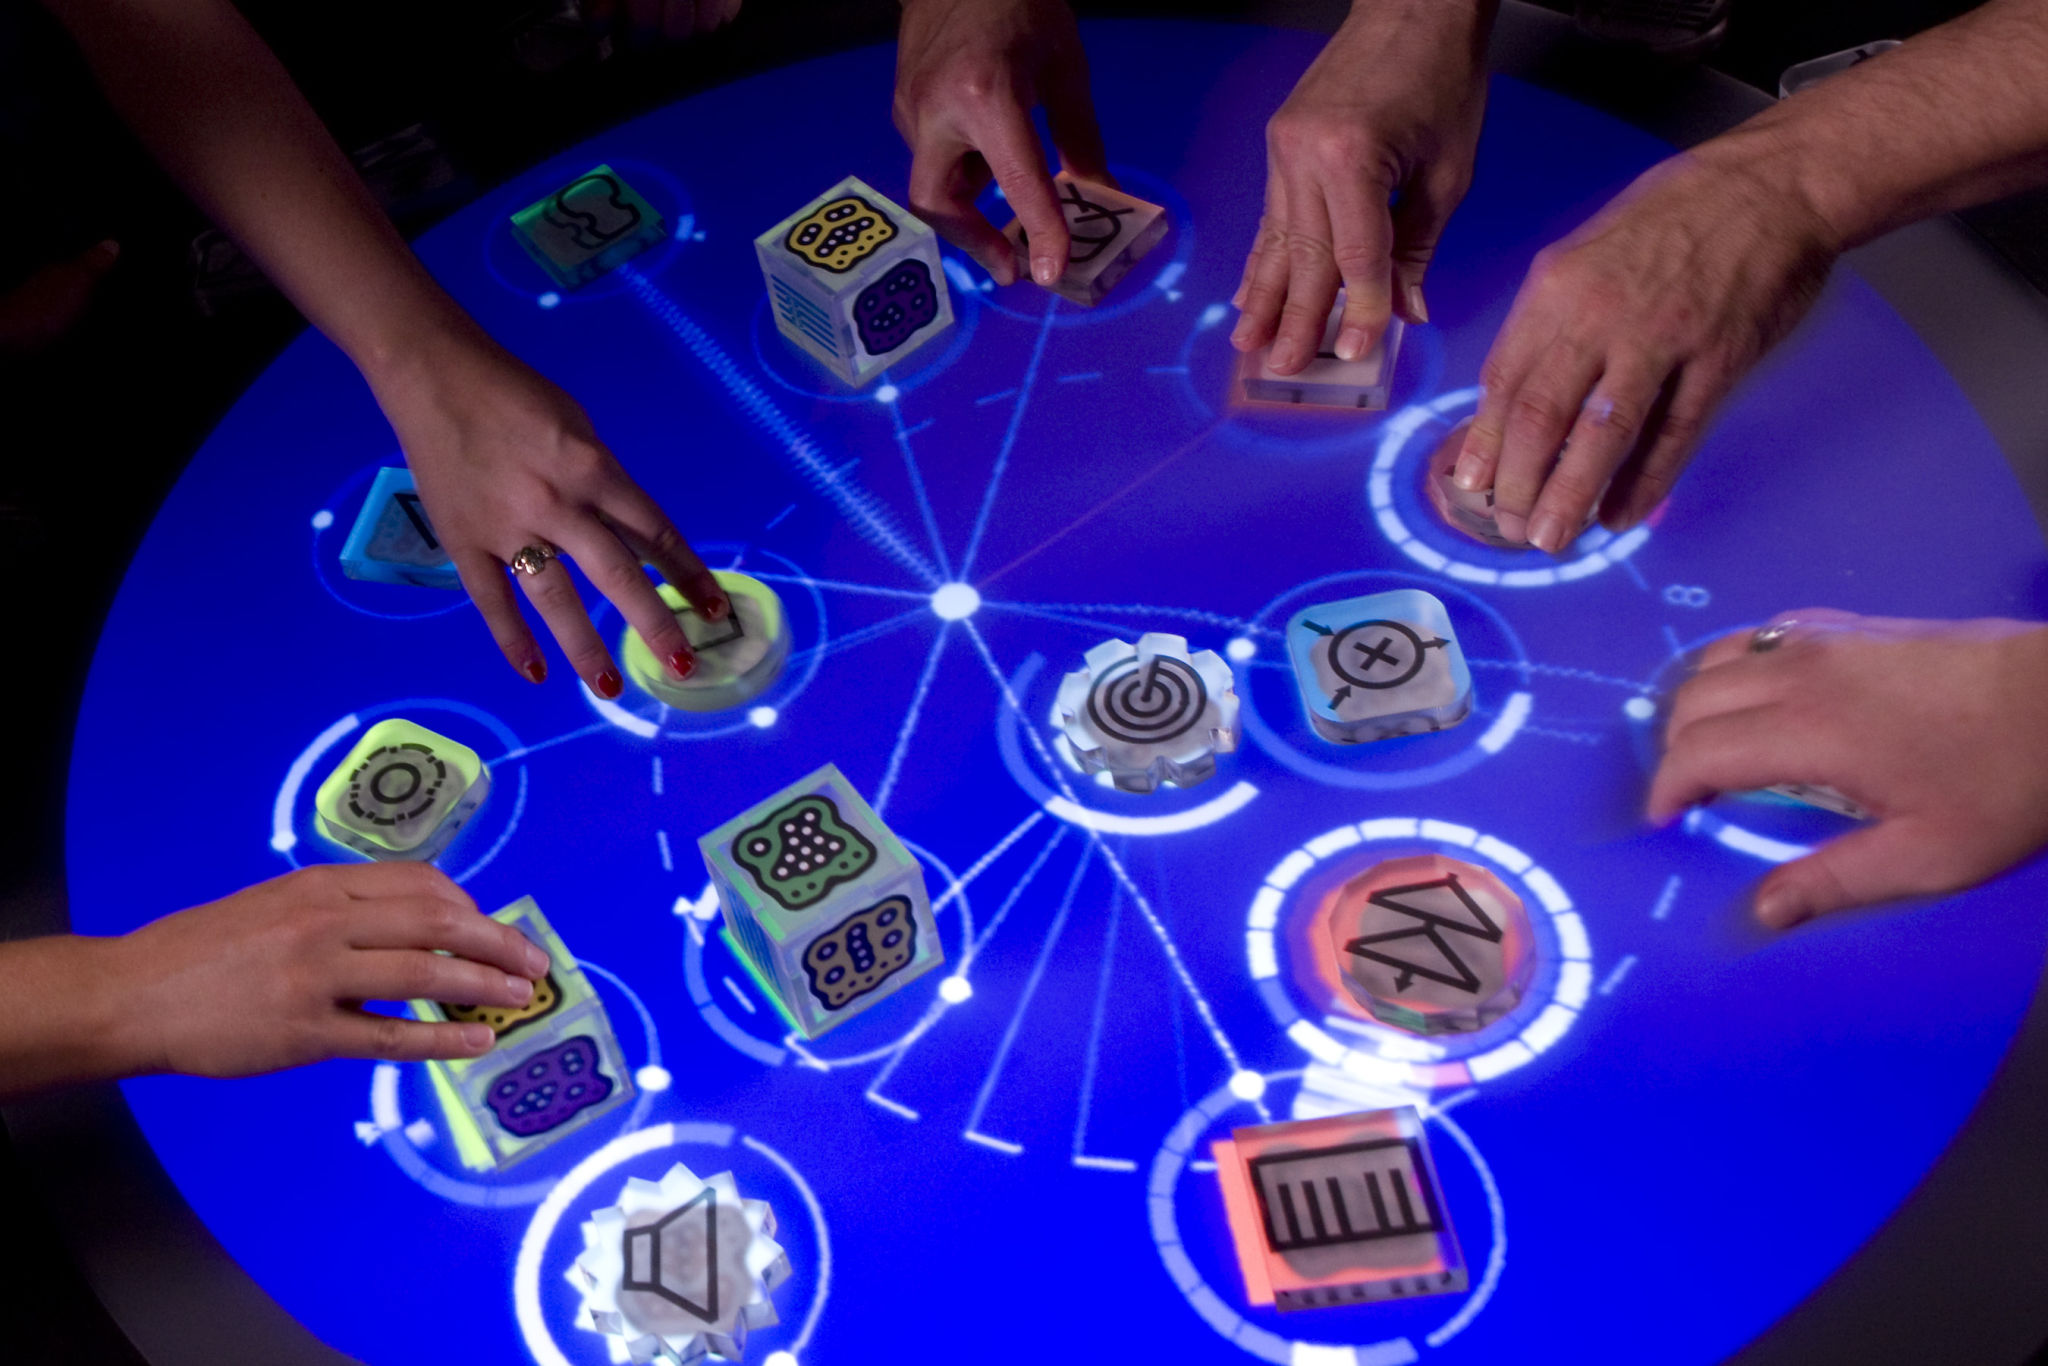
\includegraphics[width=0.6\linewidth]{figure/Analysis/reactable}
					\caption{The Reactable table synthesizer used by multiple users.}
					\label{fig:reactable}
				\end{figure} 
		
		\subsection{SketchUp}
			SketchUp\footnote{SketchUp: \url{https://www.sketchup.com/}} is a 3D modeling tool that allows for a user to create 2D lines and shapes, which can be manipulated through vertex editing turning it into 3D models in a simplistic fashion. When the 3D models are created SketchUp offers different functionalities for bringing details to the product, and then creating layout drawings from the final	model e.g. to show customers a house drawing or even landscape architecture. The software has it strengths and weaknesses in its simplicity, since it allows for intuitive modeling, but falls off on immersion making the designs seem stale. All though that could be seen as a weakness, it enables minimal memory usage to allow for a highly effortless experience. \\
			
			SketchUp exists in various versions for different professions like architecture, construction, engineering, landscape architecture and the like. Creators are enabled to share their models with the community, or save them for their own later use, to implement in bigger structure planning eg. a tree could be saved as an asset to use for a complete garden design.
			
				\begin{figure}[H]
					\centering
					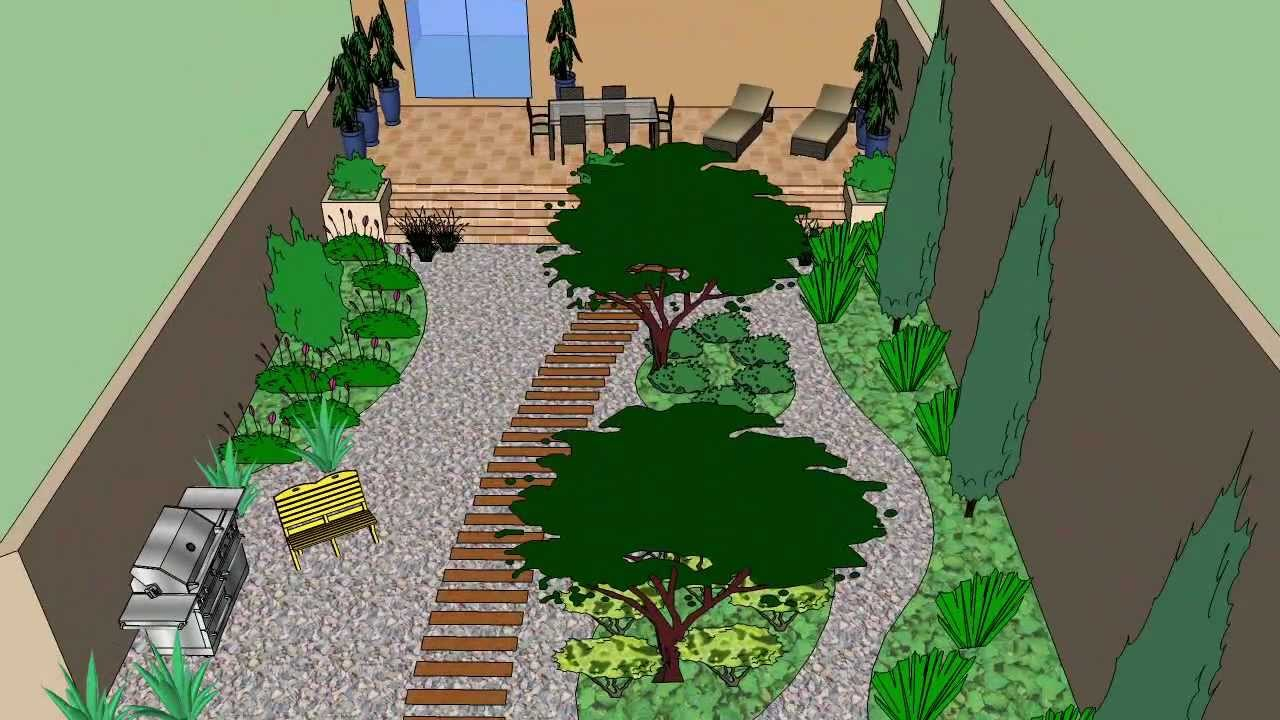
\includegraphics[width=0.6\linewidth]{figure/Analysis/sketchupgarden}
					\caption{A garden designed in SketchUp}
					\label{fig:sketchupgarden}
				\end{figure}
			
				\section{Initial Survey}
			%Plantorama surveyllama
			
			To get an initial direction which could inform further development of the project, a survey was conducted in Plantorama Hillerød, a garden centre. Of 35 respondents, 33 answered the question: How comfortable would you be trying a program utilizing "Virtual Reality"?
			
			\begin{figure}[H]
				\centering
				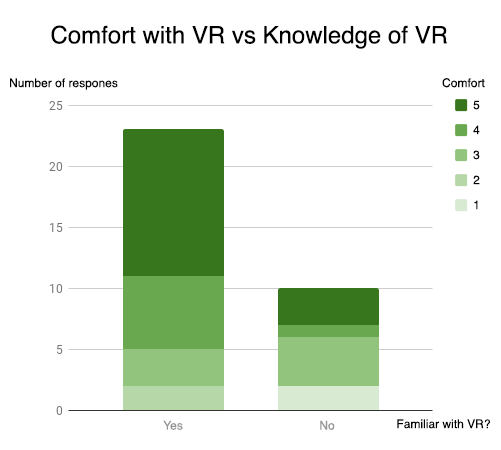
\includegraphics[width=0.6\linewidth]{figure/Analysis/comfort.png}
				\caption{How comfortable respondents were with VR according to familiarity with the technology}
				\label{fig:comfort}
			\end{figure}
			
			At first glance, a respondent's familiarity with Virtual Reality technology doesn't appear to have a great influence on their willingness to try it. However, only ten people were both unfamiliar with VR and responded to the comfort question. It is difficult to extrapolate from so little data.
			
			\begin{figure}[H]
				\centering
				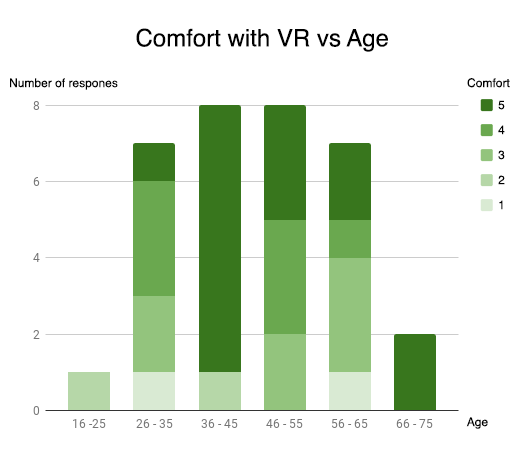
\includegraphics[width=0.6\linewidth]{figure/Analysis/vrcomfort.png}
				\caption{How comfortable respondents were with VR according to age}
				\label{fig:vrcomfort}
			\end{figure}
			
			Going in, it was expected that the younger demographic would be more comfortable with new technology than the elder. But the comfort levels of VR are actually slightly larger in the elder half of respondents. Again, this result could possibly be explained by a low number of respondents, with only one person representing the age group 16-25. Still, it appears that age does not prevent people from being comfortable trying VR.
			
			\begin{figure}[H]
				\centering
				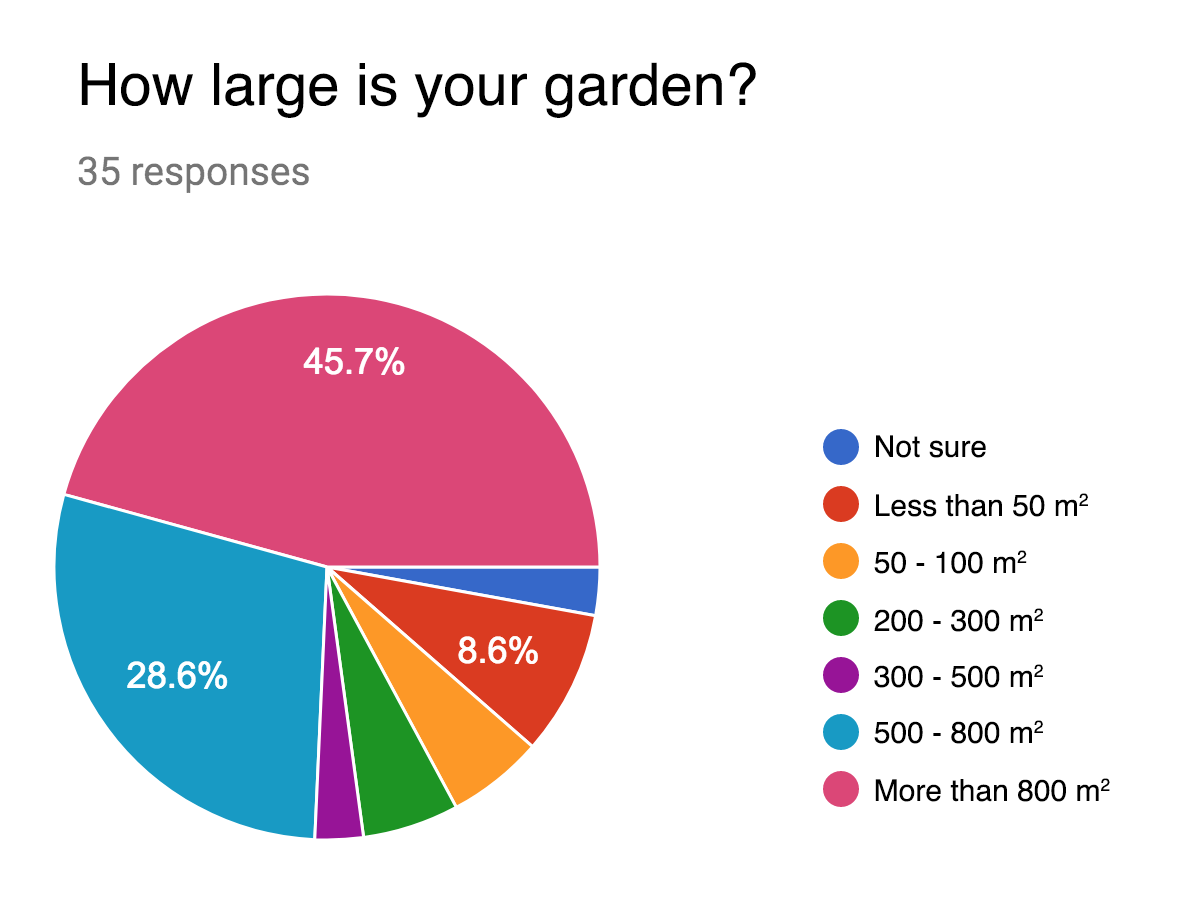
\includegraphics[width=0.6\linewidth]{figure/Analysis/gardensize.png}
				\caption{The size of respondents' gardens}
				\label{fig:gardensize}
			\end{figure}
			
			Evidently, many respondents had quite large gardens. This question would have benefited from larger size intervals and more intervals above 800 square meters.
			
			Respondents were asked to list a few of the items in their garden. Many were listed, but these were the most common answers:
			\begin{figure}[H]
				\begin{center}
					\rowcolors{2}{light-gray}{white}
					\begin{tabular}{  l  r }

						Item & Occurences  \\ \hline
						& \\
						Roses & 15 \\ 
						Rhododendron & 11  \\ 
						Apple trees & 10  \\ 
						Hydrangea & 9  \\ 
						Tulips & 5  \\ 
						Lilacs & 5  \\ 
						Strawberries & 5  \\ 
						Beech & 5  \\
					\end{tabular}
				\end{center}
				\caption{Most common plants}
				\label{fig:plantlist}
			\end{figure}
			
			If the project ends up being limited in the number of models included, it would make sense to at least include these common garden plants.
			\section{Design Requirements}
			%Some design requirements.
				\subsection{Functional requirements}
					What it should do\\
					\begin{itemize}
						\item The product should be pleasurable to use by the end user.
						\item The product should be useful, usable and accessible for the end user.
						\item The product should require only little effort from the end user's clients.
						\item It should be easy to add objects to the virtual representation of the proposed garden.
						\item The virtual environment should be pleasant to be in.
						\item the virtual environment should strive to feel immersive and realistic to the client inside it.
						
						\item The program should have enough variety in it's selection of plants to satisfy the architect's creative needs for a standard danish garden.				
						\item The architect must have control over the virtual objects' position and rotation using the physical tokens.
					\end{itemize}
					
				\subsection{Non-functional requirements}
					How it should do it\\
					\begin{itemize}
						\item User must be able to enter a virtual environment with a representation of the proposed garden using a VR headset.
						\item User must be able to walk and look around in the virtual environment.
						\item The application should include the most common plants found in a Danish garden:
						\begin{itemize}
							\item Roses
							\item Rhododendron
							\item Apple trees
							\item Hydrangea
							\item Tulips
							\item Lilacs
							\item Strawberries
							\item Beech
						\end{itemize}
						\item The above plants' should be easily identifiable by the architect using it, both the physical tokens, and the virtual representations.
						\item The program should be compatible with the HTC Vive.
						\item The architect must be able to use physical tokens, to create and modify the virtual representations of the corresponding objects, while the client is in the virtual environment.
						\item Prototype must be able to function in most natural and artificial lighting conditions.
						\item Physical construction of our prototype must lightweight and easily transportable. \todo{Should strive to be? Also, if this is going to stay, then make corresponding functional requirement that calls for it}
						\item Rotation of token must rotate virtual object.
						\item The program must run at between 60 and 90 frames per seconds on a powerful laptop.

						\item Virtual garden should support garden sizes under 50 m$^2$ and up to 1600 m$^2$.\todo{What's feasable when considering size of tokens and size of acrylic surface?}

						\item Object recognition may not fail more than 1 out of 20 times.\todo{What is the actual rate at which our product is considered bad?}
						\item Physical tokens must be easy to match to their virtual counterpart.
						\item The program must be able to handle up to 100 items \todo{How many do we actually need? Maybe as many tokens as will fit on the board?}in the virtual garden without crashing
						
						\item Virtual objects must move in real time as physical tokens are moved.
						\item Virtual objects must not exhibit a noticeable jitter
						\item Virtual object's position must correspond exactly to that of their physical token
					\end{itemize}
			